\paragraph{1. 1. Use the 1D finite-volume solver that you 
    already developed for the last problem set to solve 
    the following 1D isothermal hydrodynamics problem: the 
    $x$-grid goes from $x=-1$ to $x=1$ and it is divided 
    into $N_x=100$ cells, the boundary conditions are 
    periodic and the isothermal sound speed is $c_s=1$. 
} \ \\
    \\
    The initial conditions are 
    \begin{align}
        \rho(x, t=0)
        &=1+\varepsilon\exp\bigg(
            -\frac{x^2}{2\sigma^2}
        \bigg) \\
        u(x,t=0)
        &=0
    \end{align}
    where $\varepsilon=10^{-4}$ and $\sigma=0.2$. 
    Use CFL=0.4. \\
    \\
    For the integration, we utilize the pre-written 
    code made available on the Moodle website. First, we 
    need to do the parameter initialization. \\
    \lstinputlisting[lastline=23]{../code/task01.py} \ \\
    Next, we'd like to implement a function that allows us 
    to easily get $\rho(x)$ and $u(x)$ for various 
    integration times $t_\textnormal{max}$. For this, the 
    code base is expanded by the following: \\
    \lstinputlisting[firstline=27,lastline=37]{../code/task01.py}

\paragraph{2. How do you expect the system to physically 
    evolve? Why?
} \ \\
    \\
    If our expectations are valid, the initially very
    localized density distribution will disperse, i.e. 
    spread out. For high values of $t_\textnormal{max}$, 
    we expect the density to equalize across $x$. The 
    density $\rho(x)$ approximates a constant value that 
    is independent of location. \\
    \\
    Due to the periodic boundary conditions, the 
    distribution does not just spread out into 
    infinity, and $\rho(x)$ does not fall monotonously
    with time. Instead, the boundary conditions lead to 
    a periodic reappearance of the initial distribution's
    structure (on time scale $t_{c_s}$).

\paragraph{3. What is the value of the sound crossing 
    time scale $t_{c_s}$ for this setup?
} \ \\
    \\
    To find $t_{c_s}$, we calculate $\rho(x=0)$ for 
    various values of $t_\textnormal{max}$. Plotting them,
    the sound crossing time scale can be determined by 
    averaging over the distance between two peaks of 
    the periodic structure: \\
    \lstinputlisting[firstline=40, lastline=56]{../code/task01.py} \ \\
    This yields
    $$t_{c_s}\approx7.727$$
    \begin{figure}[h!]
        \centering
        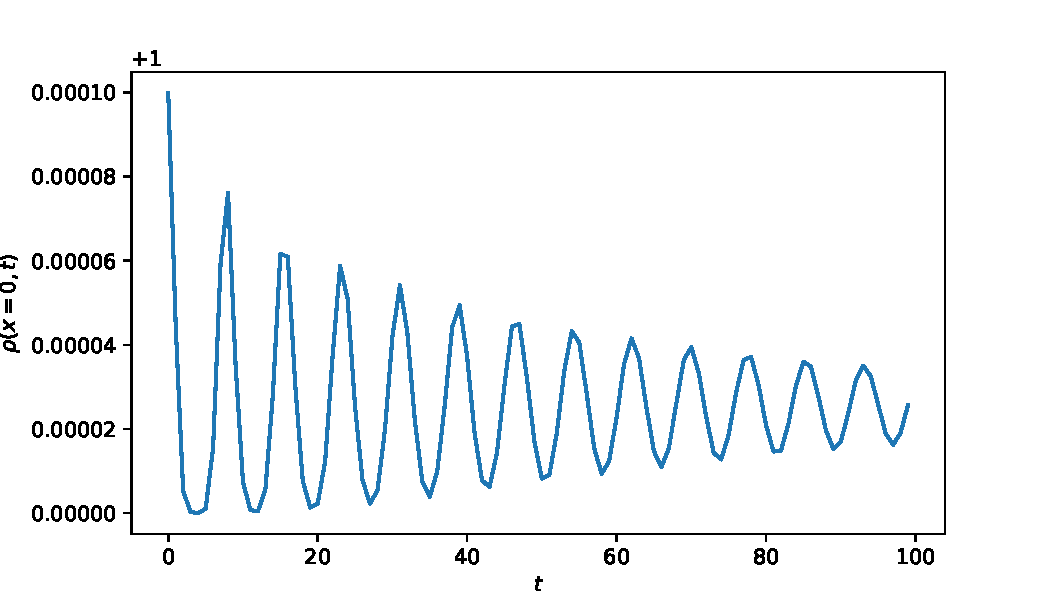
\includegraphics[width=.7\textwidth]{../figures/sound_crossing_time_scale.pdf}
    \end{figure} 

\paragraph{4. Overplot 
    $\rho(x,0)$ and $\rho(x,t^{*})$ for 
    $t^{*}=(1,2,3,4,5,6,7,8,9,10)\times t_{c_s}$. You will 
    need these overplots to make a qualitative comparison, 
    so don’t worry if you didn’t store the output exactly 
    at $t^{*}$, also the previous or the following time 
    step will be fine.
} \ \\
    \\
    Python code for getting density distribution for 
    different values of $t_\textnormal{max}$ and 
    plotting them: \\
    \lstinputlisting[firstline=62, lastline=72]{../code/task01.py} \ \\
    Resulting plot:
    \begin{figure}[h!]
        \centering
        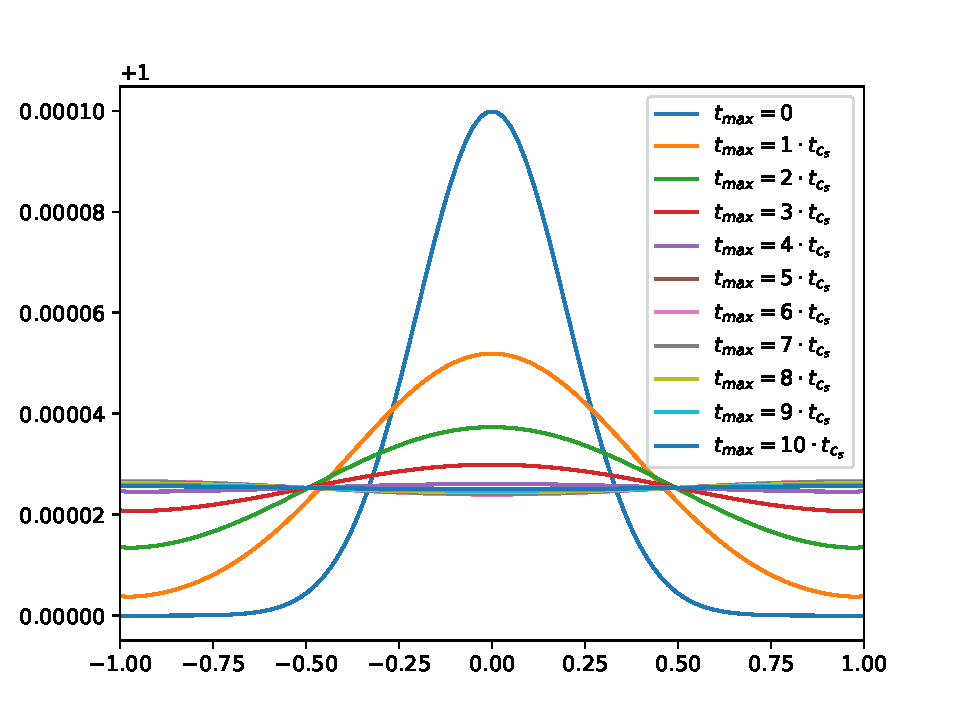
\includegraphics[width=.7\textwidth]{../figures/density_evolution.pdf}
    \end{figure} \ \\ 
    As one can see here, our expecation about the
    long-term behavior of the density distribution seems
    to be correct. The bell curve flattens and the 
    peak at $x=0$ drops off. Due to the periodic 
    dropoff behavior of the system, when looking at 
    the time dependence it is important to use mutliples 
    of the sound crossing time scale, otherwise this 
    graph would look very different.

\newpage
\paragraph{5. Plot the time evolution of the total kinetic 
    energy until $t_\textnormal{max}=10\times t_{c_s}$.
} \ \\  
    \\
    The (volume-normalized) kinetic energy can be 
    calculated from 
    \begin{equation}
        E_\textnormal{kin}=\frac{1}{2}\rho u^2
    \end{equation}
    We do this for every cell and take the sum: \\
    \lstinputlisting[firstline=74]{../code/task01.py} \ \\
    The result can be seen below:
    \begin{figure}[h!]
        \centering
        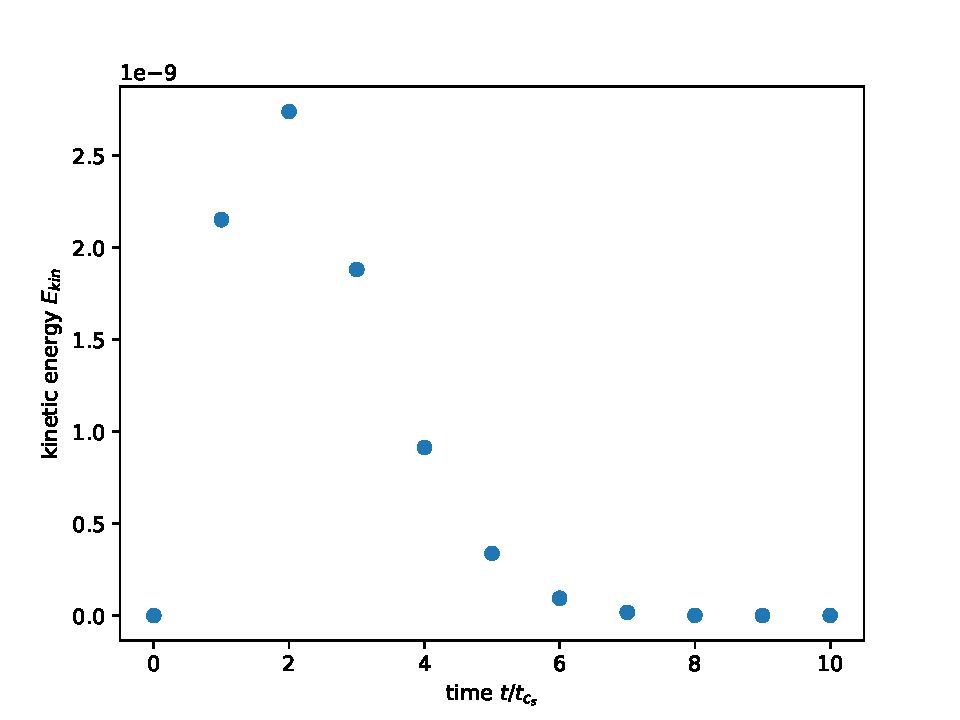
\includegraphics[width=.7\textwidth]{../figures/energy_evolution.pdf}
    \end{figure} \ \\ 
